% Options for packages loaded elsewhere
\PassOptionsToPackage{unicode}{hyperref}
\PassOptionsToPackage{hyphens}{url}
%
\documentclass[
]{article}
\usepackage{lmodern}
\usepackage{amssymb,amsmath}
\usepackage{ifxetex,ifluatex}
\ifnum 0\ifxetex 1\fi\ifluatex 1\fi=0 % if pdftex
  \usepackage[T1]{fontenc}
  \usepackage[utf8]{inputenc}
  \usepackage{textcomp} % provide euro and other symbols
\else % if luatex or xetex
  \usepackage{unicode-math}
  \defaultfontfeatures{Scale=MatchLowercase}
  \defaultfontfeatures[\rmfamily]{Ligatures=TeX,Scale=1}
\fi
% Use upquote if available, for straight quotes in verbatim environments
\IfFileExists{upquote.sty}{\usepackage{upquote}}{}
\IfFileExists{microtype.sty}{% use microtype if available
  \usepackage[]{microtype}
  \UseMicrotypeSet[protrusion]{basicmath} % disable protrusion for tt fonts
}{}
\makeatletter
\@ifundefined{KOMAClassName}{% if non-KOMA class
  \IfFileExists{parskip.sty}{%
    \usepackage{parskip}
  }{% else
    \setlength{\parindent}{0pt}
    \setlength{\parskip}{6pt plus 2pt minus 1pt}}
}{% if KOMA class
  \KOMAoptions{parskip=half}}
\makeatother
\usepackage{xcolor}
\IfFileExists{xurl.sty}{\usepackage{xurl}}{} % add URL line breaks if available
\IfFileExists{bookmark.sty}{\usepackage{bookmark}}{\usepackage{hyperref}}
\hypersetup{
  pdftitle={CS 402 Homework 1},
  pdfauthor={Muhammad Umar},
  hidelinks,
  pdfcreator={LaTeX via pandoc}}
\urlstyle{same} % disable monospaced font for URLs
\usepackage[margin=1in]{geometry}
\usepackage{color}
\usepackage{fancyvrb}
\newcommand{\VerbBar}{|}
\newcommand{\VERB}{\Verb[commandchars=\\\{\}]}
\DefineVerbatimEnvironment{Highlighting}{Verbatim}{commandchars=\\\{\}}
% Add ',fontsize=\small' for more characters per line
\usepackage{framed}
\definecolor{shadecolor}{RGB}{248,248,248}
\newenvironment{Shaded}{\begin{snugshade}}{\end{snugshade}}
\newcommand{\AlertTok}[1]{\textcolor[rgb]{0.94,0.16,0.16}{#1}}
\newcommand{\AnnotationTok}[1]{\textcolor[rgb]{0.56,0.35,0.01}{\textbf{\textit{#1}}}}
\newcommand{\AttributeTok}[1]{\textcolor[rgb]{0.77,0.63,0.00}{#1}}
\newcommand{\BaseNTok}[1]{\textcolor[rgb]{0.00,0.00,0.81}{#1}}
\newcommand{\BuiltInTok}[1]{#1}
\newcommand{\CharTok}[1]{\textcolor[rgb]{0.31,0.60,0.02}{#1}}
\newcommand{\CommentTok}[1]{\textcolor[rgb]{0.56,0.35,0.01}{\textit{#1}}}
\newcommand{\CommentVarTok}[1]{\textcolor[rgb]{0.56,0.35,0.01}{\textbf{\textit{#1}}}}
\newcommand{\ConstantTok}[1]{\textcolor[rgb]{0.00,0.00,0.00}{#1}}
\newcommand{\ControlFlowTok}[1]{\textcolor[rgb]{0.13,0.29,0.53}{\textbf{#1}}}
\newcommand{\DataTypeTok}[1]{\textcolor[rgb]{0.13,0.29,0.53}{#1}}
\newcommand{\DecValTok}[1]{\textcolor[rgb]{0.00,0.00,0.81}{#1}}
\newcommand{\DocumentationTok}[1]{\textcolor[rgb]{0.56,0.35,0.01}{\textbf{\textit{#1}}}}
\newcommand{\ErrorTok}[1]{\textcolor[rgb]{0.64,0.00,0.00}{\textbf{#1}}}
\newcommand{\ExtensionTok}[1]{#1}
\newcommand{\FloatTok}[1]{\textcolor[rgb]{0.00,0.00,0.81}{#1}}
\newcommand{\FunctionTok}[1]{\textcolor[rgb]{0.00,0.00,0.00}{#1}}
\newcommand{\ImportTok}[1]{#1}
\newcommand{\InformationTok}[1]{\textcolor[rgb]{0.56,0.35,0.01}{\textbf{\textit{#1}}}}
\newcommand{\KeywordTok}[1]{\textcolor[rgb]{0.13,0.29,0.53}{\textbf{#1}}}
\newcommand{\NormalTok}[1]{#1}
\newcommand{\OperatorTok}[1]{\textcolor[rgb]{0.81,0.36,0.00}{\textbf{#1}}}
\newcommand{\OtherTok}[1]{\textcolor[rgb]{0.56,0.35,0.01}{#1}}
\newcommand{\PreprocessorTok}[1]{\textcolor[rgb]{0.56,0.35,0.01}{\textit{#1}}}
\newcommand{\RegionMarkerTok}[1]{#1}
\newcommand{\SpecialCharTok}[1]{\textcolor[rgb]{0.00,0.00,0.00}{#1}}
\newcommand{\SpecialStringTok}[1]{\textcolor[rgb]{0.31,0.60,0.02}{#1}}
\newcommand{\StringTok}[1]{\textcolor[rgb]{0.31,0.60,0.02}{#1}}
\newcommand{\VariableTok}[1]{\textcolor[rgb]{0.00,0.00,0.00}{#1}}
\newcommand{\VerbatimStringTok}[1]{\textcolor[rgb]{0.31,0.60,0.02}{#1}}
\newcommand{\WarningTok}[1]{\textcolor[rgb]{0.56,0.35,0.01}{\textbf{\textit{#1}}}}
\usepackage{longtable,booktabs}
% Correct order of tables after \paragraph or \subparagraph
\usepackage{etoolbox}
\makeatletter
\patchcmd\longtable{\par}{\if@noskipsec\mbox{}\fi\par}{}{}
\makeatother
% Allow footnotes in longtable head/foot
\IfFileExists{footnotehyper.sty}{\usepackage{footnotehyper}}{\usepackage{footnote}}
\makesavenoteenv{longtable}
\usepackage{graphicx,grffile}
\makeatletter
\def\maxwidth{\ifdim\Gin@nat@width>\linewidth\linewidth\else\Gin@nat@width\fi}
\def\maxheight{\ifdim\Gin@nat@height>\textheight\textheight\else\Gin@nat@height\fi}
\makeatother
% Scale images if necessary, so that they will not overflow the page
% margins by default, and it is still possible to overwrite the defaults
% using explicit options in \includegraphics[width, height, ...]{}
\setkeys{Gin}{width=\maxwidth,height=\maxheight,keepaspectratio}
% Set default figure placement to htbp
\makeatletter
\def\fps@figure{htbp}
\makeatother
\setlength{\emergencystretch}{3em} % prevent overfull lines
\providecommand{\tightlist}{%
  \setlength{\itemsep}{0pt}\setlength{\parskip}{0pt}}
\setcounter{secnumdepth}{-\maxdimen} % remove section numbering
\usepackage{fancyhdr}
\usepackage{lastpage}
\pagestyle{fancy}
\fancyhead[L]{Muhammad Umar}
\fancypagestyle{plain}{}
\chead{\thepage\ / \pageref{LastPage}}
\fancyhead[R]{Homework \#1}
\lfoot{cs402 V02 Fall 2020}
\rfoot{Illinois Institute of Technology - Computer Science}
\cfoot{}

\title{CS 402 Homework 1}
\author{Muhammad Umar}
\date{}

\begin{document}
\maketitle

\hypertarget{question-1}{%
\paragraph{Question 1}\label{question-1}}

\hypertarget{a-using-trace-files-i.e.-files-that-contain-addresses-issued-by-some-cpu-to-execute-some-applications-draw-the-histogram-of-address-distribution-for-each-of-them-2x20-points.-on-the-ox-axis-of-the-plot-you-will-have-the-address-number-dont-start-with-zero-rather-with-the-smallest-address-you-find-in-the-file-and-go-up-to-the-maximum-address-in-the-file.-on-the-oy-axis-you-will-have-the-number-of-occurrences-for-each-particular-address.}{%
\subparagraph{(a) Using trace files, i.e.~files that contain addresses
issued by some CPU to execute some application(s), draw the histogram of
address distribution for each of them (2x20 points). On the Ox axis of
the plot you will have the address number (don't start with zero, rather
with the smallest address you find in the file and go up to the maximum
address in the file). On the Oy axis you will have the number of
occurrences for each particular
address.}\label{a-using-trace-files-i.e.-files-that-contain-addresses-issued-by-some-cpu-to-execute-some-applications-draw-the-histogram-of-address-distribution-for-each-of-them-2x20-points.-on-the-ox-axis-of-the-plot-you-will-have-the-address-number-dont-start-with-zero-rather-with-the-smallest-address-you-find-in-the-file-and-go-up-to-the-maximum-address-in-the-file.-on-the-oy-axis-you-will-have-the-number-of-occurrences-for-each-particular-address.}}

Spice.din

\begin{Shaded}
\begin{Highlighting}[]
\NormalTok{data1 <-}\StringTok{ }\KeywordTok{read.csv}\NormalTok{(}\StringTok{"spice.din"}\NormalTok{, }\DataTypeTok{sep=}\StringTok{" "}\NormalTok{,}\DataTypeTok{header=}\NormalTok{F, }\DataTypeTok{stringsAsFactors =}\NormalTok{ F)}
\NormalTok{addressFreq1 <-}\StringTok{ }\KeywordTok{table}\NormalTok{(data1[,}\DecValTok{2}\NormalTok{])}
\KeywordTok{barplot}\NormalTok{(addressFreq1, }\DataTypeTok{main=}\StringTok{"Frequency of address operations in Spice"}\NormalTok{, }
        \DataTypeTok{xlab =} \StringTok{"Address"}\NormalTok{, }\DataTypeTok{ylab =} \StringTok{"Access Count"}\NormalTok{)}
\end{Highlighting}
\end{Shaded}

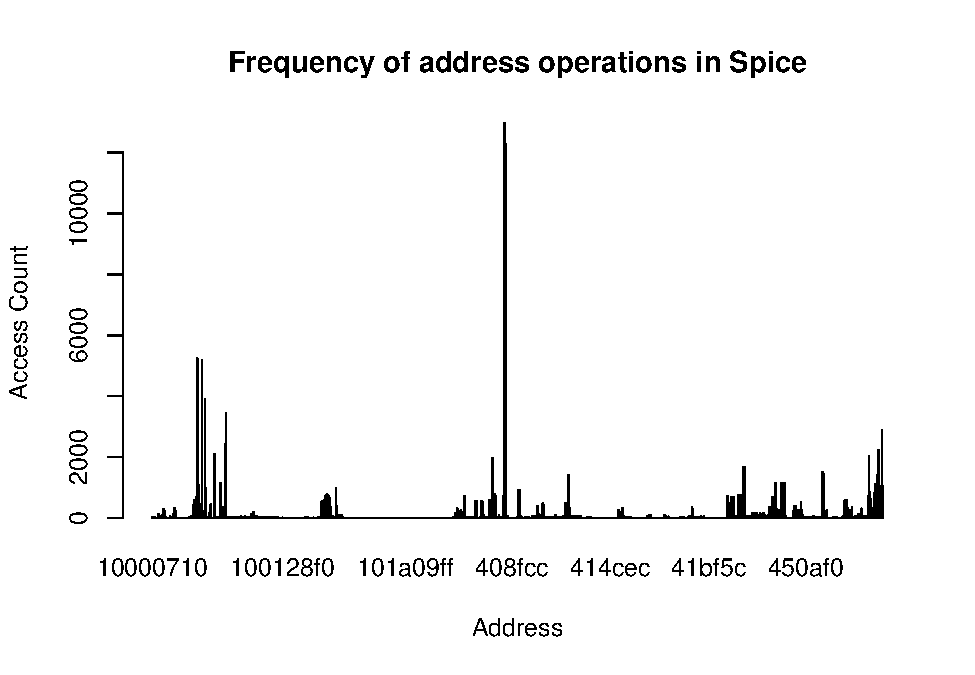
\includegraphics{muhammad-umar-hw1-cs402_files/figure-latex/unnamed-chunk-1-1.pdf}

Tex.din

\begin{Shaded}
\begin{Highlighting}[]
\NormalTok{data2 <-}\StringTok{ }\KeywordTok{read.csv}\NormalTok{(}\StringTok{"tex.din"}\NormalTok{, }\DataTypeTok{sep=}\StringTok{" "}\NormalTok{,}\DataTypeTok{header=}\NormalTok{F, }\DataTypeTok{stringsAsFactors =}\NormalTok{ F)}
\NormalTok{addressFreq2 <-}\StringTok{ }\KeywordTok{table}\NormalTok{(data1[,}\DecValTok{2}\NormalTok{])}
\KeywordTok{barplot}\NormalTok{(addressFreq2, }\DataTypeTok{main=}\StringTok{"Frequency of address operations in Tex"}\NormalTok{, }
        \DataTypeTok{xlab =} \StringTok{"Address"}\NormalTok{, }\DataTypeTok{ylab =} \StringTok{"Access Count"}\NormalTok{)}
\end{Highlighting}
\end{Shaded}

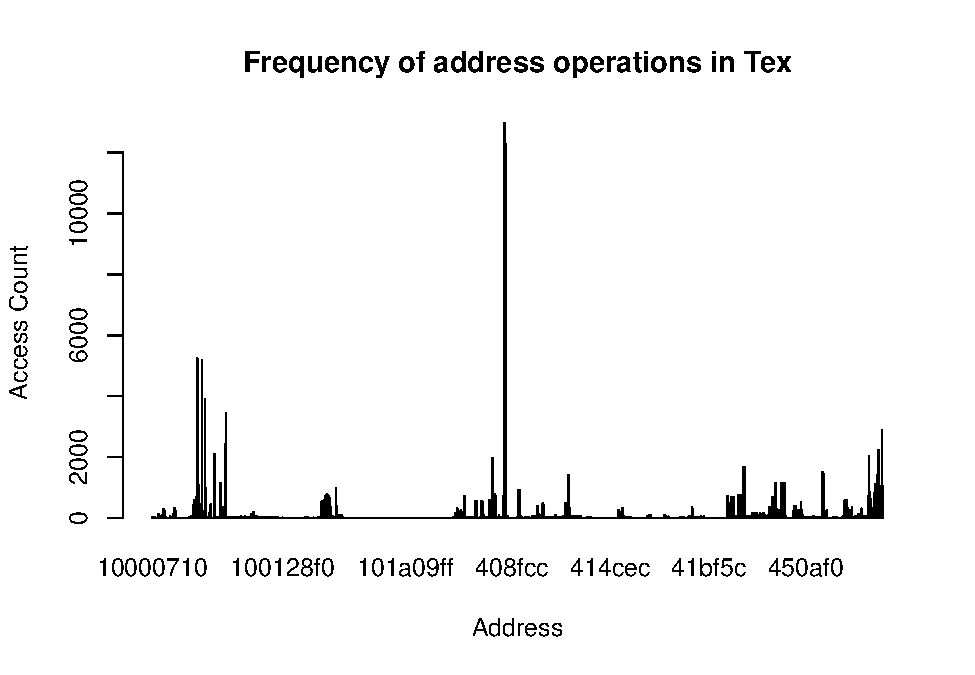
\includegraphics{muhammad-umar-hw1-cs402_files/figure-latex/unnamed-chunk-2-1.pdf}

\hypertarget{comment-based-on-the-histograms-5.}{%
\subparagraph{Comment based on the histograms
(5).}\label{comment-based-on-the-histograms-5.}}

\begin{Shaded}
\begin{Highlighting}[]
\CommentTok{# Sort as frequency table as descending and fetch the first name}
\NormalTok{spiceMaxName<-}\KeywordTok{names}\NormalTok{(}\KeywordTok{sort}\NormalTok{(}\OperatorTok{-}\KeywordTok{table}\NormalTok{(data1[,}\DecValTok{2}\NormalTok{])))[}\DecValTok{1}\NormalTok{]}
\NormalTok{texMaxName<-}\KeywordTok{names}\NormalTok{(}\KeywordTok{sort}\NormalTok{(}\OperatorTok{-}\KeywordTok{table}\NormalTok{(data2[,}\DecValTok{2}\NormalTok{])))[}\DecValTok{1}\NormalTok{]}
\end{Highlighting}
\end{Shaded}

The most highest operation count for an address in spice.din was
0x407d6c while for tex.din, it was 0x432838, although the bar plots look
very similar for both.

\hypertarget{b-what-is-the-frequency-of-writes-5-what-is-the-frequency-of-reads-5}{%
\subparagraph{(b) What is the frequency of writes (5)? What is the
frequency of reads
(5)?}\label{b-what-is-the-frequency-of-writes-5-what-is-the-frequency-of-reads-5}}

Spice.din

\begin{Shaded}
\begin{Highlighting}[]
\NormalTok{x1<-data1}\OperatorTok{$}\NormalTok{V1}
\NormalTok{maxX1<-}\KeywordTok{max}\NormalTok{(}\KeywordTok{table}\NormalTok{(x1))}
\NormalTok{\{bp1 <-}\StringTok{ }\KeywordTok{barplot}\NormalTok{(}
  \KeywordTok{table}\NormalTok{(data1}\OperatorTok{$}\NormalTok{V1), }\DataTypeTok{xaxt=}\StringTok{"n"}\NormalTok{, }\DataTypeTok{main=}\StringTok{"Frequency of operations in Spice"}\NormalTok{,}
  \DataTypeTok{ylim=}\NormalTok{(}\KeywordTok{c}\NormalTok{(}\DecValTok{0}\NormalTok{,maxX1)), }\DataTypeTok{xlab=}\StringTok{"Operation"}\NormalTok{, }\DataTypeTok{ylab=}\StringTok{"Frequency"}
\NormalTok{  )}
  \KeywordTok{axis}\NormalTok{(}\DecValTok{1}\NormalTok{, }\DataTypeTok{at=}\DecValTok{1}\OperatorTok{:}\DecValTok{3}\NormalTok{, }\DataTypeTok{labels=}\KeywordTok{c}\NormalTok{(}\StringTok{"Read"}\NormalTok{,}\StringTok{"Write"}\NormalTok{,}\StringTok{"Fetch"}\NormalTok{))}
  \KeywordTok{options}\NormalTok{(}\DataTypeTok{scipen =} \DecValTok{6}\NormalTok{)}
  \KeywordTok{text}\NormalTok{(}\DataTypeTok{x=}\NormalTok{bp1, }\DataTypeTok{y=} \KeywordTok{table}\NormalTok{(x1)}\OperatorTok{/}\DecValTok{2}\NormalTok{, }\DataTypeTok{labels=}\KeywordTok{as.character}\NormalTok{(}\KeywordTok{table}\NormalTok{(x1)))}
\NormalTok{\}}
\end{Highlighting}
\end{Shaded}

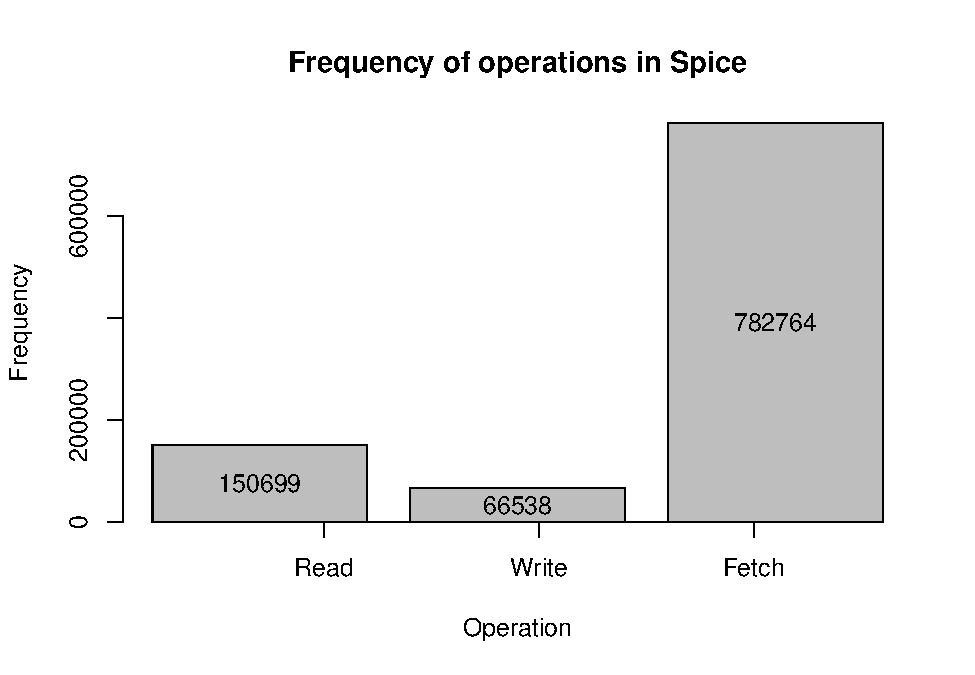
\includegraphics{muhammad-umar-hw1-cs402_files/figure-latex/unnamed-chunk-4-1.pdf}
The frequency of writes is 66538 while the frequency of reads is 150699
in the spice file.

Tex.din

\begin{Shaded}
\begin{Highlighting}[]
\NormalTok{x2<-data2}\OperatorTok{$}\NormalTok{V1}
\NormalTok{maxX2<-}\KeywordTok{max}\NormalTok{(}\KeywordTok{table}\NormalTok{(x2))}
\NormalTok{\{bp2 <-}\StringTok{ }\KeywordTok{barplot}\NormalTok{(}
  \KeywordTok{table}\NormalTok{(data2}\OperatorTok{$}\NormalTok{V1), }\DataTypeTok{main=}\StringTok{"Frequency of operations in Tex"}\NormalTok{,}
  \DataTypeTok{xlab=}\StringTok{"Operation"}\NormalTok{, }\DataTypeTok{ylab=}\StringTok{"Frequency"}\NormalTok{, }\DataTypeTok{xaxt=}\StringTok{"n"}
\NormalTok{  )}
  \KeywordTok{options}\NormalTok{(}\DataTypeTok{scipen =} \DecValTok{5}\NormalTok{)}
  \KeywordTok{axis}\NormalTok{(}\DecValTok{1}\NormalTok{, }\DataTypeTok{at=}\DecValTok{1}\OperatorTok{:}\DecValTok{3}\NormalTok{, }\DataTypeTok{labels=}\KeywordTok{c}\NormalTok{(}\StringTok{"Read"}\NormalTok{,}\StringTok{"Write"}\NormalTok{,}\StringTok{"Fetch"}\NormalTok{))}
  \KeywordTok{text}\NormalTok{(}\DataTypeTok{x=}\NormalTok{bp2, }\DataTypeTok{y=} \KeywordTok{table}\NormalTok{(x2)}\OperatorTok{/}\DecValTok{2}\NormalTok{, }\DataTypeTok{labels=}\KeywordTok{as.character}\NormalTok{(}\KeywordTok{table}\NormalTok{(x2)))}
\NormalTok{\}}
\end{Highlighting}
\end{Shaded}

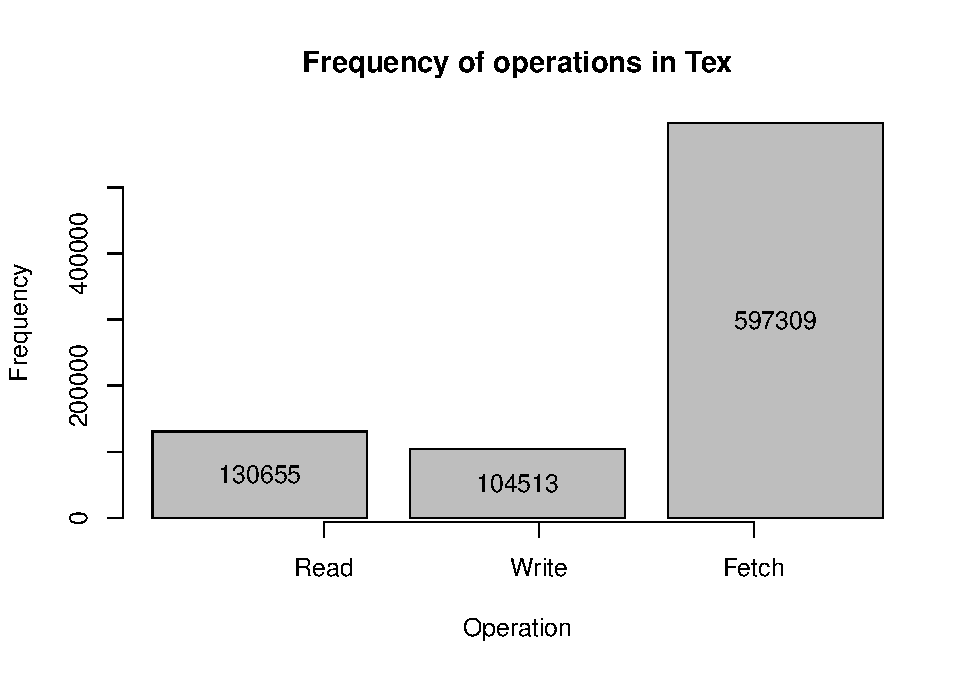
\includegraphics{muhammad-umar-hw1-cs402_files/figure-latex/unnamed-chunk-5-1.pdf}
The frequency of writes is 66538 while the frequency of reads is 150699
in the tex file.

\hypertarget{please-comment-on-these-results-5.}{%
\subparagraph{Please comment on these results
(5).}\label{please-comment-on-these-results-5.}}

Both spice.din and tex.din files show that instruction fetch was the
most common operation with spice having 782764 operations and tex having
597309 operations. They both have more read operations than write as
well. This makes sense as they address has to be fetched regardless of
whether read or write will be performed and it is common to read the
value, then perform some computation or mutate it accordingly then write
it again on either the same or other address.

\hypertarget{question-2}{%
\paragraph{Question 2}\label{question-2}}

\hypertarget{a-write-a-program-using-your-favorite-programming-language-that-multiplies-two-rectangular-matrices-please-no-square-matrices-whose-elements-are-randomly-generated.-you-will-have-two-versions-of-the-program-one-in-which-matrix-elements-are-integers-and-another-one-where-they-are-real-numbers-double-2x15-points.-measure-the-time-it-takes-each-program-to-complete-2x5-and-then-compare-the-performance-of-the-two-systems-5.}{%
\subparagraph{(a) Write a program, using your favorite programming
language, that multiplies two rectangular matrices -- please no square
matrices -- whose elements are randomly generated. You will have two
versions of the program, one in which matrix elements are integers and
another one where they are real numbers (double) (2x15 points). Measure
the time it takes each program to complete (2x5) and then compare the
performance of the two systems
(5).}\label{a-write-a-program-using-your-favorite-programming-language-that-multiplies-two-rectangular-matrices-please-no-square-matrices-whose-elements-are-randomly-generated.-you-will-have-two-versions-of-the-program-one-in-which-matrix-elements-are-integers-and-another-one-where-they-are-real-numbers-double-2x15-points.-measure-the-time-it-takes-each-program-to-complete-2x5-and-then-compare-the-performance-of-the-two-systems-5.}}

\begin{table}
\caption{\label{tab:unnamed-chunk-6}Machine 1 vs Machine 2 time taken in seconds}

\centering
\begin{tabular}[t]{r|r|r}
\hline
Runs & Integer & Float\\
\hline
1 & 4.96672 & 5.70465\\
\hline
2 & 5.29337 & 5.20660\\
\hline
3 & 5.33969 & 5.51428\\
\hline
4 & 5.05501 & 5.34071\\
\hline
5 & 5.34676 & 5.58114\\
\hline
6 & 5.02560 & 5.48730\\
\hline
7 & 5.39096 & 5.60357\\
\hline
8 & 5.41396 & 5.64611\\
\hline
9 & 5.37972 & 5.73424\\
\hline
10 & 5.26595 & 5.46428\\
\hline
\end{tabular}
\centering
\begin{tabular}[t]{r|r|r}
\hline
Runs & Integer & Float\\
\hline
1 & 6.73228 & 7.62045\\
\hline
2 & 6.66859 & 7.11992\\
\hline
3 & 7.09571 & 6.77833\\
\hline
4 & 7.21846 & 7.00182\\
\hline
5 & 7.44075 & 6.97693\\
\hline
6 & 7.10797 & 7.28310\\
\hline
7 & 7.33325 & 6.87675\\
\hline
8 & 6.88468 & 6.80096\\
\hline
9 & 6.89846 & 7.76262\\
\hline
10 & 6.84239 & 6.87293\\
\hline
\end{tabular}
\end{table}

Performance Comparison

\begin{longtable}[]{@{}lrr@{}}
\toprule
Matrix Type & Machine 1 Average & Machine 2 Average\tabularnewline
\midrule
\endhead
Integer & 5.247774 & 7.022254\tabularnewline
Float & 5.528288 & 7.109381\tabularnewline
\bottomrule
\end{longtable}

On average, Integer operations are 28.3\% slower on the 2nd machine
while float operations are 37.8\% slower.

\hypertarget{is-the-performance-ratio-the-same-as-the-clock-rate-ratio-of-the-two-systems-5-explain.}{%
\subparagraph{Is the performance ratio the same as the clock rate ratio
of the two systems (5)?
Explain.}\label{is-the-performance-ratio-the-same-as-the-clock-rate-ratio-of-the-two-systems-5-explain.}}

No, the clock speed of the first machine is 150\% greater (3.3 GHz
versus 2.2 Ghz of the second) while the difference in performance is
less than 40\% on average.

This is because clock speeds are not the determining factor of computer
performance but cycles per instruction is. Other factors such as
available cache, type of storage (NVME SSD vs SATA SSD), type of RAM
depending on architecture (DDR4 vs LPDDR3) all affect cycles per
instruction.

\hypertarget{based-on-the-retail-price-of-the-two-systems-which-one-is-more-cost-effective-5}{%
\subparagraph{Based on the retail price of the two systems, which one is
more cost effective
(5)?}\label{based-on-the-retail-price-of-the-two-systems-which-one-is-more-cost-effective-5}}

The first machine is a GT73VR with a Skylake i7 (6th generation) running
at 3.3GHz clock speed with a M2 NVMe SSD and costs approximately
\$\$1500 today. The second machine is a 15 inch Macbook Pro 2015
equipped with a Broadwell i7 (5th generation) running at 2.2Ghz clock
speed with a M2 SSD and costs approximately \$1100 today.

The first machine is 36\% more expensive while the difference of
performance is greater than 38\%.

Hence, the first machine (MSI GT73VR) is more cost effective.

\hypertarget{b-change-your-multiplication-algorithm-and-repeat-the-steps-above-for-instance-if-you-used-the-the-naive-multiplication-algorith-with-the-column-in-the-inner-loop-then-just-use-the-same-algorithm-with-the-row-in-the-inner-loop-same-scoring-as-part-a.}{%
\subparagraph{(b) Change your multiplication algorithm and repeat the
steps above; for instance, if you used the the naive multiplication
algorith with the column in the inner loop, then just use the same
algorithm with the row in the inner loop (same scoring as part
a).}\label{b-change-your-multiplication-algorithm-and-repeat-the-steps-above-for-instance-if-you-used-the-the-naive-multiplication-algorith-with-the-column-in-the-inner-loop-then-just-use-the-same-algorithm-with-the-row-in-the-inner-loop-same-scoring-as-part-a.}}

\begin{table}
\caption{\label{tab:unnamed-chunk-8}Machine 1 vs Machine 2 time taken in seconds (rows in inner loop)}

\centering
\begin{tabular}[t]{r|r|r}
\hline
Runs & Integer & Float\\
\hline
1 & 4.80913 & 5.40437\\
\hline
2 & 5.23265 & 5.16091\\
\hline
3 & 4.88205 & 4.99780\\
\hline
4 & 5.08705 & 5.22991\\
\hline
5 & 5.04049 & 5.07952\\
\hline
6 & 5.10803 & 5.24946\\
\hline
7 & 5.11938 & 5.42984\\
\hline
8 & 5.13538 & 5.33022\\
\hline
9 & 5.06068 & 5.28904\\
\hline
10 & 5.28394 & 5.30617\\
\hline
\end{tabular}
\centering
\begin{tabular}[t]{r|r|r}
\hline
Runs & Integer & Float\\
\hline
1 & 6.75647 & 7.42215\\
\hline
2 & 7.34534 & 7.28856\\
\hline
3 & 6.89118 & 7.33798\\
\hline
4 & 6.97223 & 7.11317\\
\hline
5 & 7.05036 & 7.36661\\
\hline
6 & 6.91155 & 7.57345\\
\hline
7 & 6.76589 & 7.48034\\
\hline
8 & 6.73468 & 7.48641\\
\hline
9 & 7.58147 & 7.50841\\
\hline
10 & 6.96372 & 7.38413\\
\hline
\end{tabular}
\end{table}

Performance Comparison

\begin{longtable}[]{@{}lrr@{}}
\toprule
Matrix Type & Machine 1 Average & Machine 2 Average\tabularnewline
\midrule
\endhead
Integer & 5.075878 & 6.997289\tabularnewline
Float & 5.247724 & 7.396121\tabularnewline
\bottomrule
\end{longtable}

On average, Integer operations are 37.85\% slower on the 2nd machine
while float operations are 40.94\% slower.

\hypertarget{machine-description}{%
\subparagraph{Machine Description}\label{machine-description}}

\begin{longtable}[]{@{}lll@{}}
\toprule
Attribute & Machine 1 & Machine 2\tabularnewline
\midrule
\endhead
Manufacturer & MSI & Apple\tabularnewline
CPU Type & i7-6820HK & i7 Broadwell (5th generation)\tabularnewline
Clock Speed & 3.3GHz & 2.2 GHz\tabularnewline
RAM & 32GB & 16 GB\tabularnewline
OS & Windows 10 & macOS Catalina\tabularnewline
Compiler & G++ MinGW & LLVM-g++\tabularnewline
SSD Random Read Speeds & 39.24 MB/s & 19.27 MB/s\tabularnewline
SSD Random Write Speeds & 88.6 MB/s & 30.98 MB/s\tabularnewline
Price & \$1,500 & \$1100\tabularnewline
\bottomrule
\end{longtable}

The SSD read/write speeds were taken using Crystal Disk Mark's random
4kb read/write single-thread test

\end{document}
